\documentclass[logo,reportComp]{thesis}
\usepackage[cpp,linenum]{mypackage}

\title{计算机网络实验报告}
\subtitle{实验三:Chat实验}
\school{数据科学与计算机学院}
\author{陈鸿峥}
\classname{17大数据与人工智能}
\stunum{17341015}
\headercontext{计算机网络实验报告}

\begin{document}

\maketitle

\section{实验目的}
掌握套接字的多线程编程方法,实现多人聊天。

\section{实验介绍}
利用客户/服务器(Client/Sever或CS)模式实现一个多人聊天(群聊)程序,其功能是每个客户发送给服务器的消息都会传送给所有的客户端。
\begin{center}
\begin{tikzcd}
\text{client1}\arrow[bend left]{rrd}{\text{Hello}} & & \\
\text{client2} & & \text{server}\arrow[swap]{llu}{\text{Hello}}\arrow[swap]{ll}{\text{Hello}}\arrow{lld}{\text{Hello}}\\
\text{client3} & & 
\end{tikzcd}
\end{center}

\section{参考资料}
\begin{itemize}
	\item Introduction to Multi-Threaded Programming (Linux), \url{https://www.linuxjournal.com/article/3138}
    % \item https://www.cnblogs.com/liangf27/p/9356837.html
    % \item https://stackoverflow.com/questions/37453845/pthread-create-is-called-multiple-times-while-the-previous-thread-with-same-rout
    % \item Linux下socket通信和epoll https://www.cnblogs.com/liangf27/p/9366348.html
\end{itemize}

\section{实验环境}
本机为Ubuntu 18.04 (LTS) + gcc 7.3.0

\section{注意事项}
\begin{itemize}
    \item 依步骤完成以下实验内容,尽量多完成一些步骤
    \item 把出现的问题、解决方法和一些思考和体会写在实验体会部分
    \item 对典型的运行情况的客户和服务器控制台进行截屏并放在实验结果部分
    \item 截屏用按键(Ctrl+Alt+PrintScreen)单独截取控制台窗口。截屏应尽量windows绘图程序缩小尺寸(能看清就行)后粘入
    \item 端口号采用\textcolor{red}{50500}
    \item 字符串可以采用函数\verb'scanf'或\verb'gets'输入
\end{itemize}

\section{实验内容}
先阅读课件``套接字并发编程.PDF'',重点是读懂课件中``chat并发编程(服务器)''和``chat并发编程(客户端)''的流程图,然后完成下面步骤(截屏要同时显示服务器和至少两个客户端)。
\begin{figure}[H]
\centering
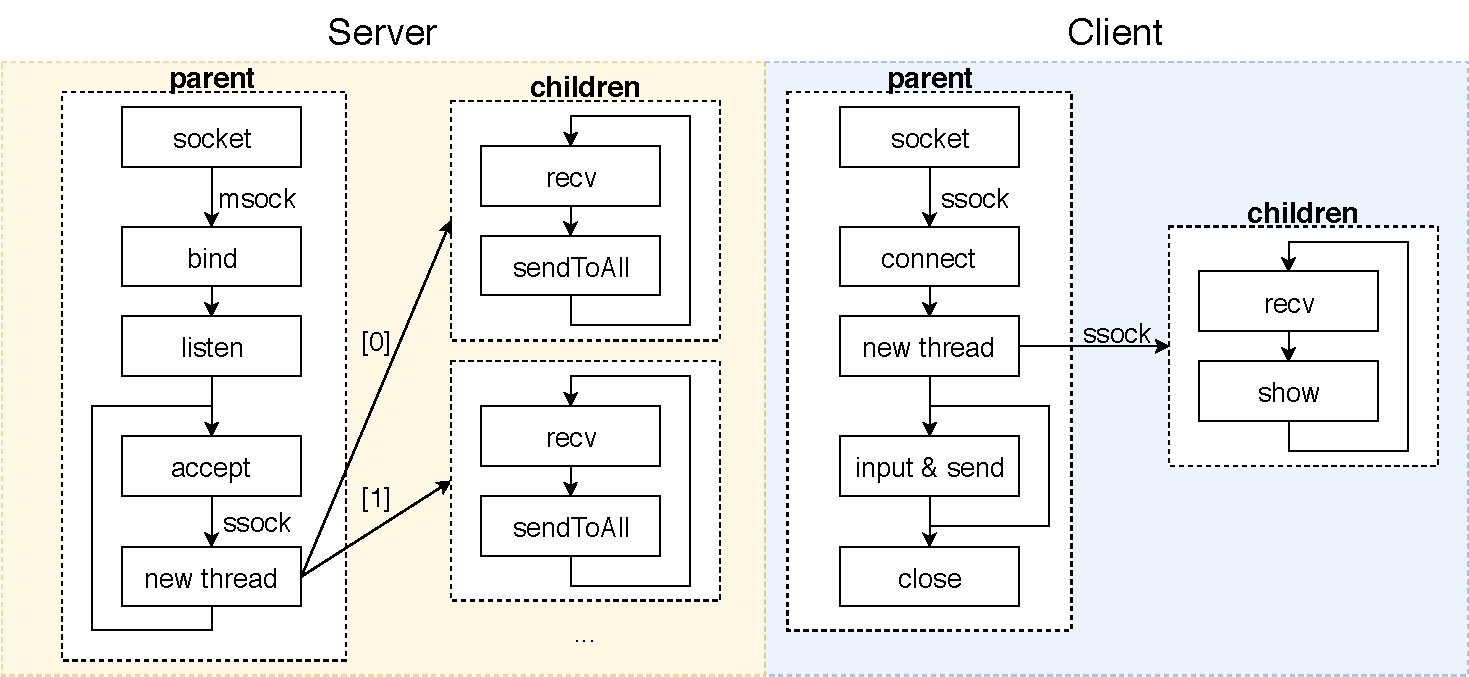
\includegraphics[width=\linewidth]{fig/socket-multithread.pdf}
\end{figure}

\subsection{多人聊天程序}
编写多人聊天程序,要求客户端和服务器都采用多线程方式进行编程。
每个客户端都采用\textbf{TCP协议}连接服务器并保持连接。
服务器同时与所有客户端建立和保持连接。
每个客户端输入的消息都会通过服务器转发给所有客户。

Linux环境下线程调用需要引入头文件\verb'<pthread.h>',同时添加编译指令\verb'-pthread'。
创建线程为\verb'pthread_create',退出线程为\verb'pthread_exit',线程等待为\verb'pthread_join'。

服务器端程序:(注意这里采用\textbf{命令行参数选择不同的问题编号},如本题运行程序传\verb'./server 1')
\begin{lstlisting}
#include <stdio.h>
#include <stdlib.h>
#include <sys/socket.h>
#include <netinet/in.h>
#include <arpa/inet.h>
#include <sys/types.h>
#include <unistd.h>
#include <string.h>
#include <error.h>
#include <time.h>
#include <pthread.h> // multi-thread

#define BUF_LEN 2000
#define MAX_CLIENT_NUM 10

void generateMsg(char* buffer){
    char buf[BUF_LEN+1];
    printf("`消息:'%s\n", buffer);
    sprintf(buf,"`消息:'%s\n",buffer);
    strcpy(buffer,buf);
}

void sendToAll(int* ssock, char* buf){
    for (int i = 0; i < MAX_CLIENT_NUM; ++i)
        if (ssock[i] != -1){
            int cc = send(ssock[i], buf, strlen(buf), 0);
        }
}

int findEmptySSock(int* ssock)
{
    for (int i = 0; i < MAX_CLIENT_NUM; ++i)
        if (ssock[i] == -1)
            return i;
    perror("No ssocks available!");
    abort();
    return -1;
}

typedef struct shared_data
{
    int index;
    int* ssock; // used for communication with each other
    int mode;
    struct in_addr client_addr;
    int port;
} shared_data;

void* serve(void* arg);

int main(int argc, char *argv[])
{
    struct  sockaddr_in fsin;               /* the from address of a client   */
    int     msock;                          /* master socket                  */
    int     ssock[MAX_CLIENT_NUM];          /* slaver sockets                 */
    char    *service = "50500";             /* port number                    */
    struct  sockaddr_in sin;                /* an Internet endpoint address   */
    int     addlen;                         /* from-address length            */

    // create socket
    msock = socket(PF_INET, SOCK_STREAM, IPPROTO_TCP);      // master sock

    memset(&sin,'\0', sizeof(sin));
    sin.sin_family = AF_INET;
    sin.sin_addr.s_addr = INADDR_ANY;
    sin.sin_port = htons((u_short)atoi(service));
    bind(msock, (struct sockaddr *)&sin, sizeof(sin));

    listen(msock, 5); // create queue

    for (int i = 0; i < MAX_CLIENT_NUM; ++i)
        ssock[i] = -1;

    printf("`服务器已启动!'\n\n");

    pthread_t pthid[MAX_CLIENT_NUM];

    shared_data sdata;
    while(1) {
        addlen = sizeof(struct sockaddr);
        // `如果在连接请求队列中有连接请求,则接受连接请求并建立连接,返回该连接的套接字'
        // `否则,本语句被阻塞直到队列非空。fsin包含客户端IP地址和端口号'
        int index = findEmptySSock(ssock);
        ssock[index] = accept(msock, (struct sockaddr *)&fsin, &addlen);// slaver sock

        sdata.index = index;
        sdata.ssock = ssock;
        if (argc > 1)
            sdata.mode = atoi(argv[1]);
        else
            sdata.mode = 1;
        sdata.client_addr = fsin.sin_addr;
        sdata.port = fsin.sin_port;
        // pthread_create(&thrd1, NULL, (void *)&thread_function, (void *) &some_argument);
        pthread_create(&pthid[index],NULL,serve,(void*)& sdata); // multi-thread
    }
    for (int i = 0; i < MAX_CLIENT_NUM; ++i)
        pthread_join(pthid[i],NULL);
    close(msock);
    return 0;
}

void* serve(void* arg)
{
    char buf[BUF_LEN+1];
    shared_data* sdata = (shared_data*) arg;
    int index = sdata->index;
    int* ssock = sdata->ssock;
    struct in_addr client_addr = sdata->client_addr;
    int port = sdata->port;
    if (sdata->mode >= 3){
        generateEnterMsg(buf, index, (unsigned char*) &client_addr, port);
        sendToAll(ssock,buf);
    }
    while (1){
        // `返回值:(>0)接收到的字节数,(=0)对方已关闭,(<0)连接出错'
        int cc = recv(ssock[index], buf, BUF_LEN, 0);
        if (cc <= 0){ // error or closed
            if (sdata->mode >= 4){
                generateExitMsg(buf,ssock,index);
                sendToAll(ssock,buf);
            }
            ssock[index] = -1; // set null
            break;
        }
        else if (cc > 0) {
            buf[cc] = '\0';

            switch (sdata->mode){
                case 1: generateMsg(buf);break;
                case 2: // problem 2
                case 3: // problem 3
                case 4: // problem 4
                default: generateMsg2(buf, (unsigned char *) &client_addr, port);break;
            }
            sendToAll(ssock,buf);
        }
    }
    close(ssock[index]);
    pthread_exit(0);
}
\end{lstlisting}

客户端程序:
\begin{lstlisting}
#include <stdio.h>
#include <stdlib.h>
#include <sys/types.h>
#include <sys/socket.h>
#include <netinet/in.h>
#include <arpa/inet.h>
#include <unistd.h>
#include <string.h>
#include <error.h>
#include <pthread.h>

#define BUF_LEN 2000

void* receive(void* arg);

int main(int argc, char *argv[])
{
    char    *host = "127.0.0.1";       /* server IP to connect         */
    char    *service = "50520";        /* server port to connect       */
    struct  sockaddr_in sin;           /* an Internet endpoint address */
    char    buf[BUF_LEN+1];            /* buffer for one line of text  */
    int     sock;                      /* socket descriptor            */
    int     cc;                        /* recv character count         */

    // create socket
    sock = socket(PF_INET, SOCK_STREAM, IPPROTO_TCP);

    printf("`正在连接服务器'...\n");
    memset(&sin, 0, sizeof(sin));
    sin.sin_family = AF_INET;
    sin.sin_addr.s_addr = inet_addr(host);
    sin.sin_port = htons((u_short)atoi(service));
    int ret = connect(sock, (struct sockaddr *)&sin, sizeof(sin));
    if (ret == 0)
        printf("`连接成功!'\n\n");
    else {
        perror("Error: `连接失败!'\n");
        abort();
    }

    pthread_t pt;
    pthread_create(&pt,NULL,receive,&sock); // multi-thread

    while (1){
        scanf("%s", buf);
        if (strcmp(buf,"exit") == 0)
            break;
        // `返回值为实际发送的字节数,出错或对方关闭时返回SOCKET\_ERROR。'
        cc = send(sock, buf, strlen(buf), 0);
        if (cc <= 0){
            perror("Error: Server!\n");
            return 0;
        }
    }

    close(sock);

    printf("`按回车键继续'...\n");
    getchar();
    return 0;
}

void* receive(void* arg)
{
    char buf[BUF_LEN+1];
    int* sock = (int*) arg;
    while (1){
        int cc = recv(*sock, buf, BUF_LEN, 0);
        if (cc <= 0){
            perror("Error: Server!\n");
            abort();
            break;
        }
        buf[cc] = '\0';
        printf("%s\n", buf);
    }
    pthread_exit(0);
}
\end{lstlisting}

在本实验中我还编写了Makefile文件,方便自动编译。
\begin{lstlisting}[language=make]
CC = gcc
FLAGS = -pthread
ALL = server client

all: $(ALL)

% : %.c
    $(CC) $(FLAGS) $< -o $@

.PHONY : clean

clean :
    -rm -f *.o $(ALL)
\end{lstlisting}

运行截屏:(上面为服务器端,下面两个为客户端)
\begin{figure}[H]
\centering
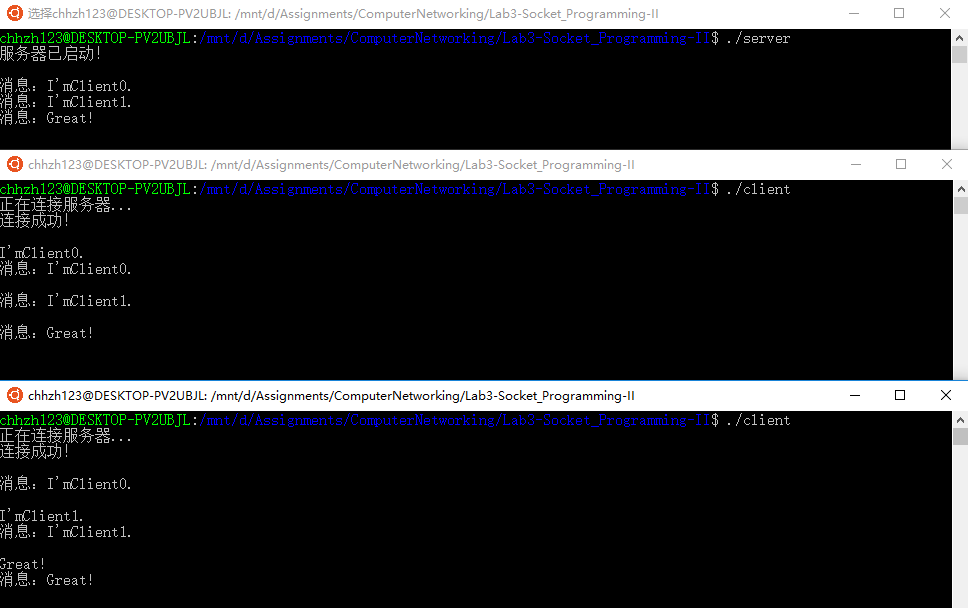
\includegraphics[width=\linewidth]{fig/p1.PNG}
\end{figure}

\subsection{添加信息后转发}
服务器程序转发某个客户端发来的消息时都在消息前面加上该客户端的IP地址和端口号以及服务器的当前时间。
要求服务器程序把转发的消息也显示出来。

服务器程序(修改部分):
\begin{lstlisting}
void generateMsg2(char* buffer, unsigned char *bytes, u_short port)
{
    char buf[BUF_LEN+1];
    // inet_ntoa
    snprintf(buf, sizeof(buf), "`客户端IP地址:'%d.%d.%d.%d\n",
              bytes[0], bytes[1], bytes[2], bytes[3]);
    printf("%s", buf);

    char buf2[BUF_LEN+1];
    sprintf(buf2, "`客户端端口号:'%d\n", port);
    printf("%s", buf2);
    strcat(buf, buf2);

    time_t now; /* current time */
    time(&now);
    char* pts = (char *)ctime(&now);
    printf("`服务器时间:'%s", pts);
    sprintf(buf2,"`服务器时间:'%s", pts);
    strcat(buf, buf2);

    printf("`收到信息:'%s\n", buffer);
    sprintf(buf2, "`内容:'%s\n", buffer);
    strcat(buf, buf2);

    printf("\n");
    strcpy(buffer,buf);
}
\end{lstlisting}

运行截屏:(上面为服务器端,下面两个为客户端)
\begin{figure}[H]
\centering
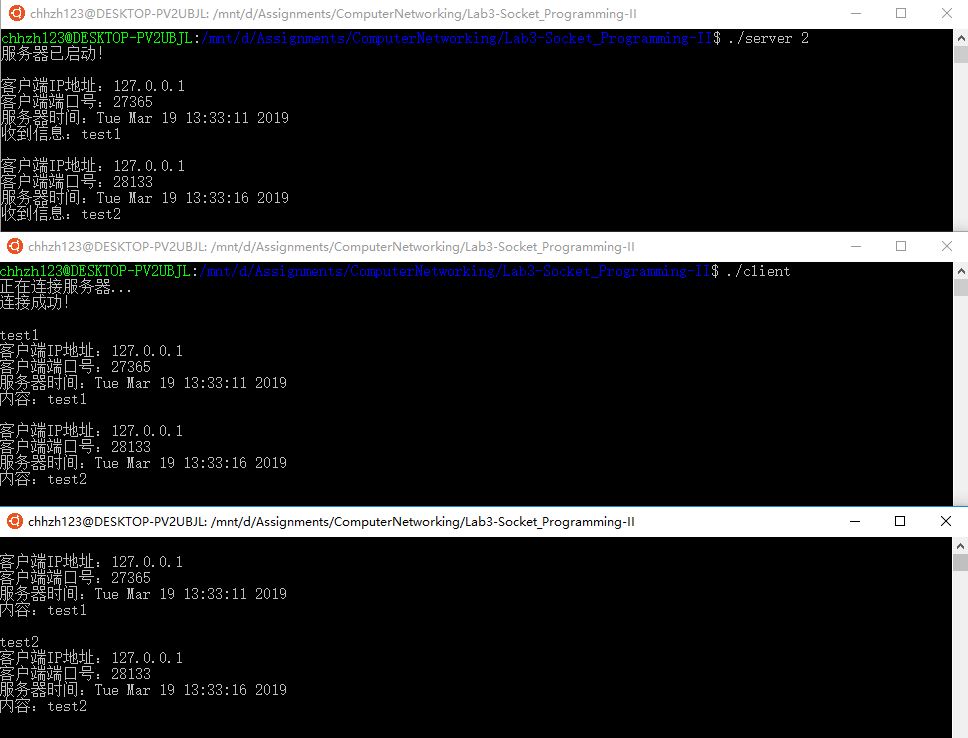
\includegraphics[width=\linewidth]{fig/p2.PNG}
\end{figure}

\subsection{``进入''信息发送}
新客户刚连接时服务器端把\verb'enter'消息(包含客户端IP地址和端口号)发送给所有客户端。

服务器程序(修改部分):
\begin{lstlisting}
void generateEnterMsg(char* buffer, int index, unsigned char *bytes, u_short port)
{
    char buf[BUF_LEN+1];
    sprintf(buf,"%d`号客户端进入'\n",index);
    printf("%s", buf);

    // inet_ntoa
    char buf2[BUF_LEN+1];
    snprintf(buf2, sizeof(buf2), "`客户端IP地址:'%d.%d.%d.%d\n",
              bytes[0], bytes[1], bytes[2], bytes[3]);
    printf("%s", buf2);
    strcat(buf,buf2);

    sprintf(buf2, "`客户端端口号:'%d\n", port);
    printf("%s", buf2);
    strcat(buf, buf2);

    strcpy(buffer,buf);
}
\end{lstlisting}

运行截屏:(上面为服务器端,下面两个为客户端)
\begin{figure}[H]
\centering
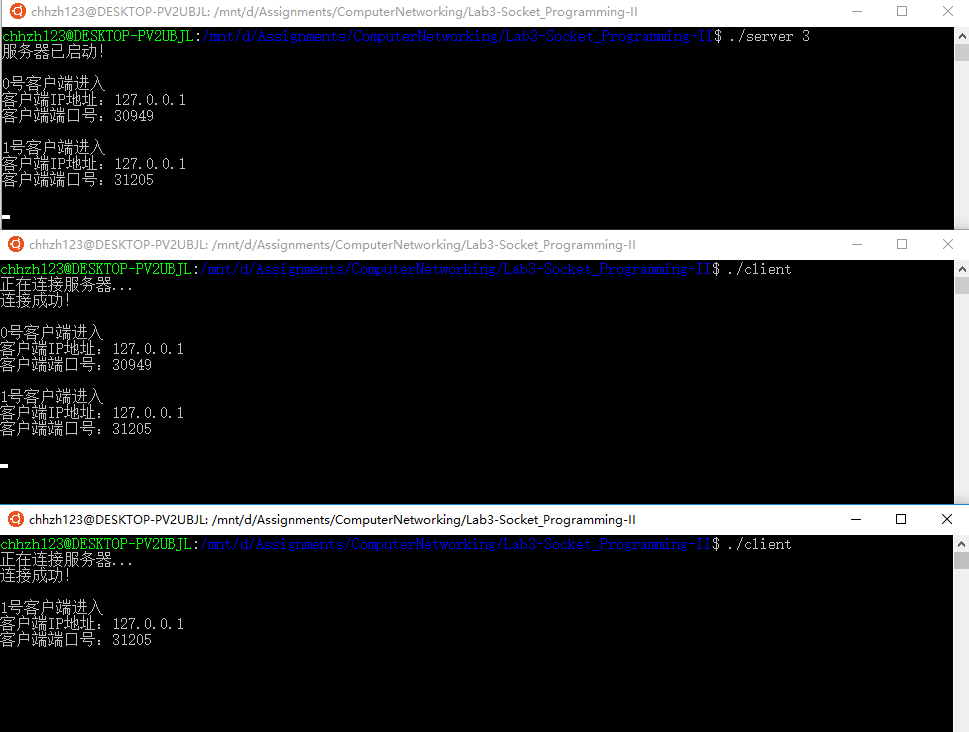
\includegraphics[width=\linewidth]{fig/p3.PNG}
\end{figure}

\subsection{``退出''信息发送}
客户端输入\verb'exit'时退出客户端程序(正常退出),或者客户端直接关闭窗口退出(异常退出),服务器都会把该客户\verb'leave'的消息广播给所有客户。

由于客户端进入时已经发送其客户端IP地址及端口号,故这里\textbf{退出时不再重复发送}。

服务器程序(修改部分):
\begin{lstlisting}
void generateExitMsg(char* buf, int* ssock, int index)
{
    sprintf(buf,"`客户端'%d`离开'!\n",index);
    printf("%s\n", buf);
}
\end{lstlisting}

运行截屏:(上面为服务器端,下面两个为客户端,其中第一个正常退出,第二个异常退出)
\begin{figure}[H]
\centering
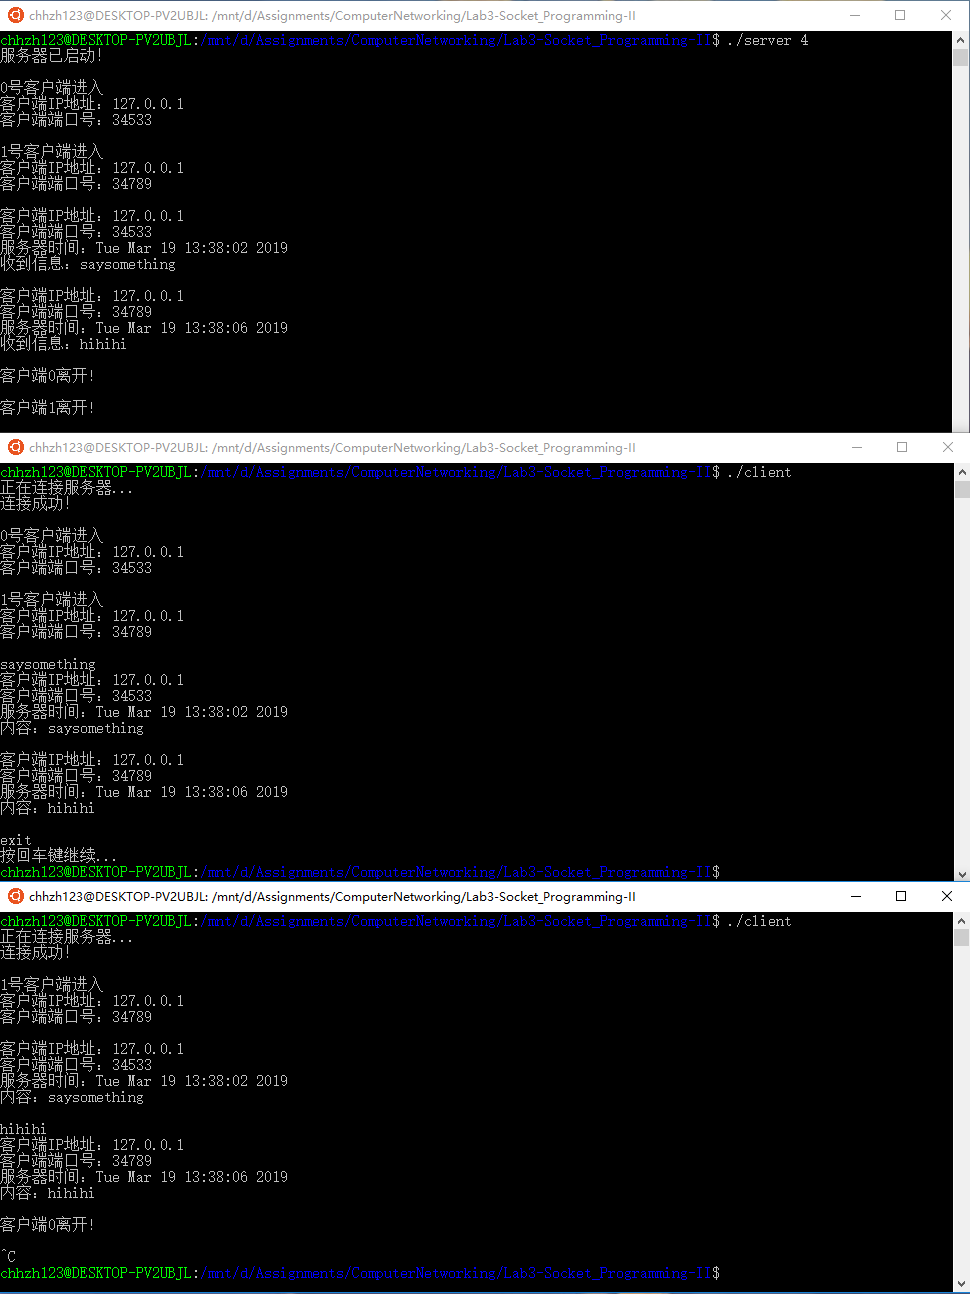
\includegraphics[width=\linewidth]{fig/p4.PNG}
\end{figure}

\subsection{与老师服务器连接}
运行客户端程序测试与老师的服务器程序的连接(\verb'172.18.187.9:50500')。

运行截屏(客户端):
\begin{figure}[H]
\centering
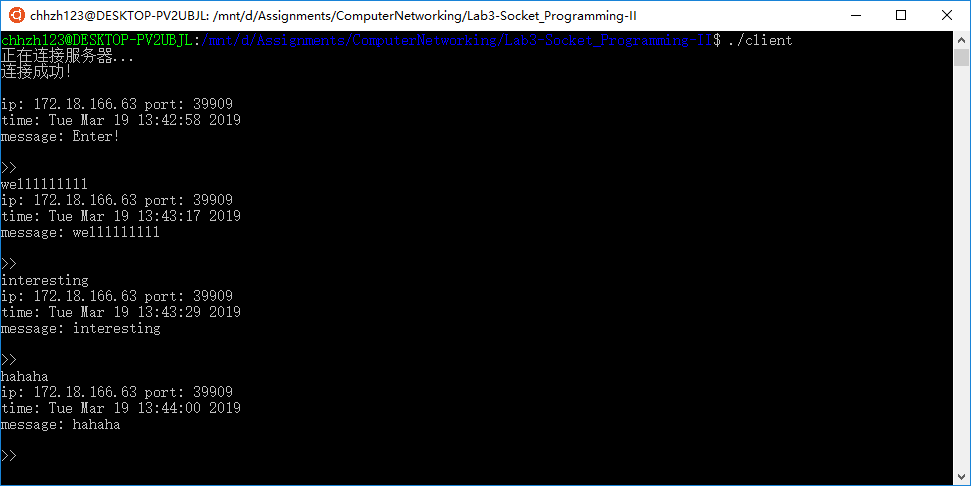
\includegraphics[width=\linewidth]{fig/p5.PNG}
\end{figure}

\subsection{与同学互测}
与同学的程序进行相互测试,一个人可以与多人测试,截屏选择其中一个。

同学的学号姓名(可以多人):17341111刘学海

作为服务器运行截屏:(注意本程序是在个人服务器上运行;并且由于互测了多次,换了多个网络,所以截图的IP地址会经常改变)
\begin{figure}[H]
\centering
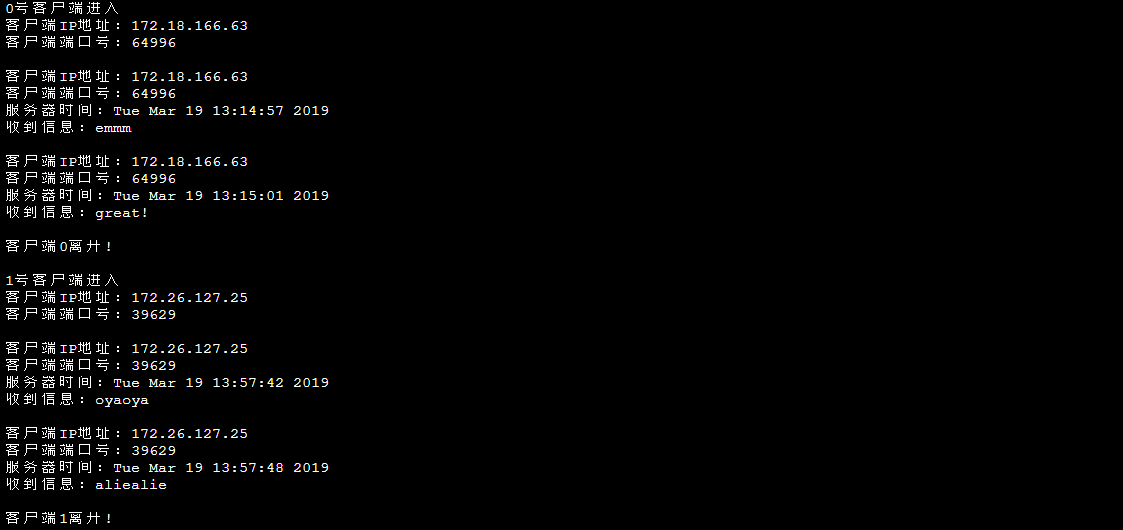
\includegraphics[width=\linewidth]{fig/cross-server.PNG}
\end{figure}

作为客户端运行截屏:
\begin{figure}[H]
\centering
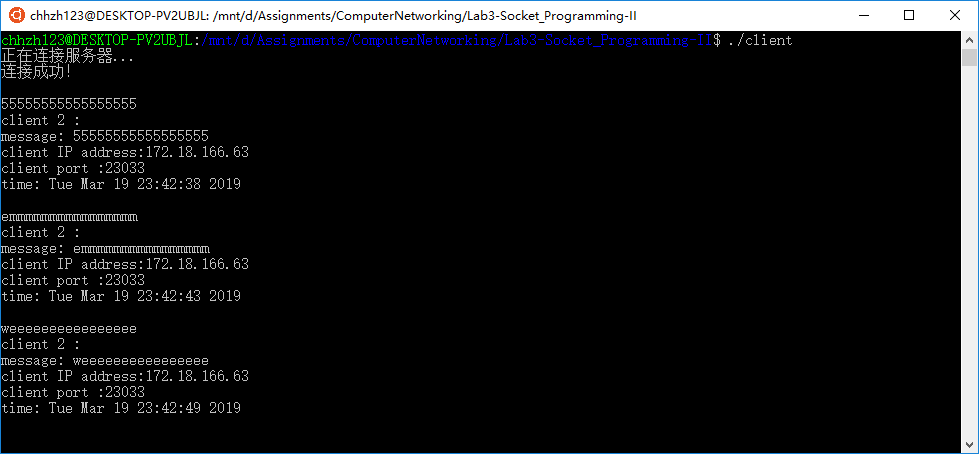
\includegraphics[width=\linewidth]{fig/cross-client.PNG}
\end{figure}


\section{完成情况}
是否完成以下步骤?(\cmark 完成\quad\xmark 未做)
\par 1. [\cmark]\qquad 2. [\cmark]\qquad 3.[\cmark]
\par 4. [\cmark]\qquad 5. [\cmark]\qquad 6.[\cmark]

\section{实验体会}
% 写出实验过程中遇到的问题,解决方法和自己的思考;并简述实验体会(如果有的话)。

本次实验非常有趣,学会了并发编程的一些基础理论,也明白如何缓解计算机网络中出现的堵塞延迟等问题。

由于有了第二次实验的基础,所以这个实验添加多线程元素并不是很复杂。
本次实验再次印证了Linux环境下的优越性,调用多线程库进行网络编程非常的方便。

自己与自己测试时基本没有出现什么问题,与同学互测却出现了很多问题。
首先是互相之间是否有办法ping通,往往由于各自电脑防火墙的缘故,导致端口并不对外开放。
查找资料并设置好防火墙就花费了很长时间。
而且由于是我的Linux系统是Windows子系统,系统内核可能存在一些bug,与同学的Windows客户端互连时会出现接不通的问题,这一点还没找到原因,最后是将我的程序放上纯Ubuntu系统的服务器才得以解决。
还有一点则是Linux和Windows环境下命令行的编码问题,常常会导致中文无法正常显示。(Windows默认GBK,Linux默认UTF-8)

总的来说,本次实验收获良多,更加深入理解了多线程编程及套接字的原理。

\end{document}
% 【交实验报告】
% 每位同学单独完成本实验内容并填写实验报告。
%     交作业地点:http://172.18.187.9/netdisk/default.aspx?vm=17net 
% 编程实验 
% 截止日期:2019年3月23日23:00(周六)。
% 上传文件:学号_姓名_chat实验报告.doc
% 学号_姓名_chat实验要求.rar (源程序和可执行程序)